\hypertarget{opc-ua-mqtt-e-sparkplug-b}{%
\chapter{OPC UA, MQTT e Sparkplug B}\label{opc-ua-mqtt-e-sparkplug-b}}

\section*{Objetivos de Aprendizagem}

Ao final deste capítulo, o leitor será capaz de:

\begin{itemize}
\tightlist
\item
  Explicar por que a integração de sistemas é um problema de \textbf{semântica}, não apenas de protocolo.
\item
  Descrever o modelo de informação do OPC UA e a função do espaço de endereços.
\item
  Distinguir os modos de segurança do OPC UA e escolher uma política adequada.
\item
  Diferenciar o OPC UA cliente-servidor do OPC UA PubSub e dizer quando cada um se aplica.
\item
  Explicar o modelo publish-subscribe do MQTT, seus níveis de QoS, \emph{retained messages} e \emph{last will}.
\item
  Descrever o que o Sparkplug B acrescenta ao MQTT e por que isso importa em IIoT.
\item
  Projetar uma integração CLP \ensuremath{\rightarrow} borda \ensuremath{\rightarrow} SCADA \ensuremath{\rightarrow} plataforma combinando os três.
\item
  Reconhecer os erros de projeto mais comuns nessas integrações.
\end{itemize}

\begin{center}\rule{0.5\linewidth}{0.5pt}\end{center}

\hypertarget{o-problema-conectar-uxe9-fuxe1cil-entender-uxe9-difuxedcil}{%
\section{O problema: conectar é fácil, entender é difícil}\label{o-problema-conectar-uxe9-fuxe1cil-entender-uxe9-difuxedcil}}

Um CLP que expõe 4.000 registradores Modbus está ``conectado''. Mas o que é o registrador 40012? É a pressão de descarga da bomba 2? Em que unidade? Está escalado? Qual o valor que significa ``sem medição''?

Essa é a diferença entre \textbf{transporte} e \textbf{semântica}:

\begin{itemize}
\tightlist
\item
  \textbf{Transporte} leva bytes de um ponto a outro: Modbus, TCP, MQTT, HTTP.
\item
  \textbf{Semântica} diz o que os bytes significam: identificação do ativo, unidade, escala, tipo de dado, qualidade, relação entre variáveis.
\end{itemize}

Modbus e outros protocolos clássicos resolvem o transporte e deixam a semântica para a documentação --- que envelhece, se perde e diverge entre projetos. OPC UA e Sparkplug B são respostas diferentes ao mesmo problema: \textbf{levar significado junto com o dado}.

\textbf{Tabela 13.1 -- Onde cada solução atua}

\begin{longtable}[]{@{}
  >{\raggedright\arraybackslash}p{(\columnwidth - 4\tabcolsep) * \real{0.3333}}
  >{\raggedright\arraybackslash}p{(\columnwidth - 4\tabcolsep) * \real{0.3333}}
  >{\raggedright\arraybackslash}p{(\columnwidth - 4\tabcolsep) * \real{0.3333}}@{}}
\toprule\noalign{}
\begin{minipage}[b]{\linewidth}\raggedright
Camada
\end{minipage} & \begin{minipage}[b]{\linewidth}\raggedright
O que define
\end{minipage} & \begin{minipage}[b]{\linewidth}\raggedright
Quem resolve bem
\end{minipage} \\
\midrule\noalign{}
\endhead
\bottomrule\noalign{}
\endlastfoot
Transporte confiável & Entrega da mensagem & TCP, MQTT, OPC UA \\
Identificação do dado & Qual variável, de qual ativo & OPC UA (espaço de endereços); Sparkplug B (tópico + métricas) \\
Significado do dado & Tipo, unidade, escala, faixa & OPC UA (modelo de informação); Sparkplug B (payload tipado) \\
Qualidade e tempo & Valor válido? De quando? & OPC UA (\emph{status code}, \emph{source timestamp}); Sparkplug B (\emph{timestamp} por métrica) \\
Comportamento & Como ler, escrever, assinar, descobrir & OPC UA (serviços); Sparkplug B (estado, nascimento/morte) \\
\end{longtable}

\begin{caixadica}

\textbf{Dica:} antes de escolher o protocolo, escreva a \textbf{lista de variáveis com unidade, faixa e regra de qualidade}. Metade dos projetos de integração falha porque essa lista não existe e a outra metade porque ela existe apenas na cabeça de quem escreveu o CLP.

\end{caixadica}

\begin{center}\rule{0.5\linewidth}{0.5pt}\end{center}

\hypertarget{opc-ua}{%
\section{OPC UA}\label{opc-ua}}

A \textbf{OPC UA} (\emph{OPC Unified Architecture}) foi lançada pela OPC Foundation em \textbf{2008} e é normalizada como a série \textbf{IEC 62541} (verifique a edição vigente antes de citá-la em projeto). Ela sucedeu o OPC clássico (DCOM) resolvendo três limitações que inviabilizavam seu uso em redes industriais modernas: dependência de Windows/DCOM, dificuldade de atravessar \emph{firewalls} e ausência de um modelo de informação padronizado.

\begin{caixanota}

\textbf{Referência histórica:} o \textbf{OPC clássico} (OPC DA, 1996) organizava o acesso a dados em
três níveis --- \textbf{servidor}, \textbf{grupo} e \textbf{item}. O grupo existia por uma razão prática: era a
unidade de \emph{scan rate} e de ativação, o que permitia ler mais devagar o que não mudava.
Referência atualmente aplicável: \textbf{OPC UA (IEC 62541)}. Motivo da atualização: o OPC clássico
depende de DCOM/Windows e não atravessa \emph{firewall} corporativo de forma segura.

\end{caixanota}

\begin{figure}
\centering
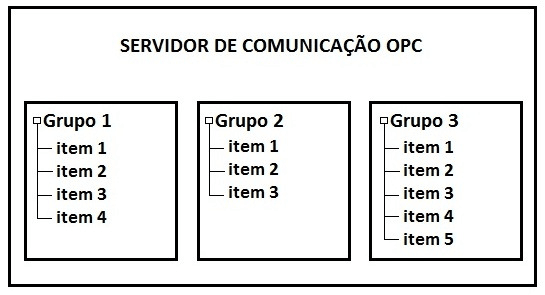
\includegraphics{../figuras/cap13-opc-arquitetura-logica.png}
\caption[Figura 13.1 -- Arquitetura lógica do OPC clássico: servidor, grupos e itens]{Figura 13.1 -- Arquitetura lógica do OPC clássico: servidor, grupos e itens. \textbf{Fonte:} \emph{Livro SCADA --- versão para análise}, p.~48 (Machado, Pontes e Vianna, reproduzida com crédito).}
\end{figure}

Vale entender essa hierarquia porque o OPC UA \textbf{manteve a ideia} e trocou a implementação: o que
no OPC clássico era ``grupo com taxa de leitura'' virou \textbf{sessão com assinatura}
(\passthrough{\lstinline!Subscription!} + \passthrough{\lstinline!MonitoredItem!}), e o ``item'' virou \textbf{nó} de um espaço de endereços com tipo,
unidade e qualidade. A herança explica por que tantos clientes OPC UA ainda expõem a leitura
``por grupo de itens'': é a tradução direta do modelo antigo.

\hypertarget{modelo-de-informauxe7uxe3o}{%
\subsection{Modelo de informação}\label{modelo-de-informauxe7uxe3o}}

O OPC UA não expõe ``registradores'': expõe um \textbf{espaço de endereços} (\emph{address space}) organizado em \textbf{nós} ligados por \textbf{referências} hierárquicas.

\begin{center}
\IfFileExists{../figuras/capitulo-13-m1.pdf}{%
  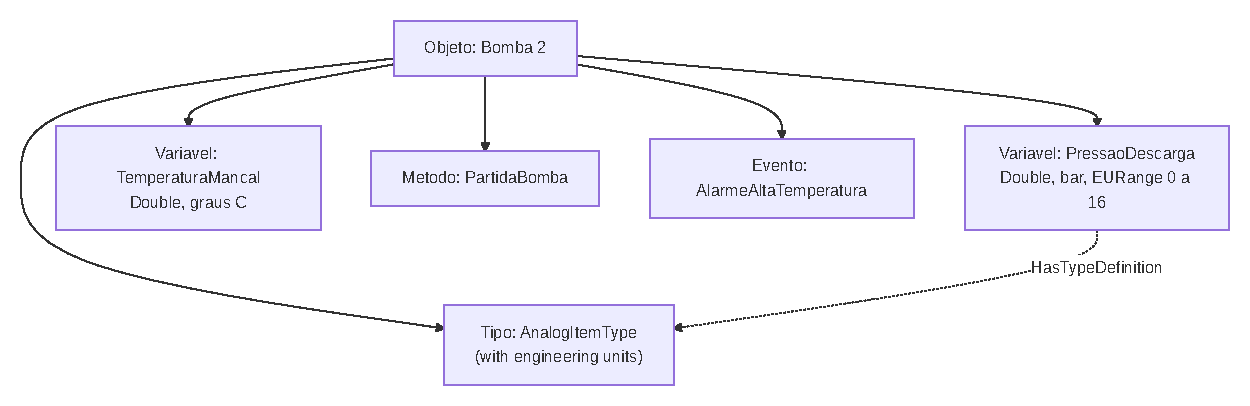
\includegraphics[width=\linewidth,height=0.8\textheight,keepaspectratio]{../figuras/capitulo-13-m1.pdf}%
}{\fbox{\parbox{0.9\linewidth}{\small Diagrama Mermaid ainda não renderizado: capitulo-13-m1. Rode scripts/render-mermaid.sh.}}}
\end{center}

Cada nó tem \textbf{atributos} (valor, tipo, \emph{status code}, \emph{source timestamp}, descrição) e \textbf{referências} para outros nós. A hierarquia é definida pelo servidor, não pelo cliente --- o cliente \textbf{descobre} a estrutura com \passthrough{\lstinline!Browse!} em vez de receber um mapa de registradores.

Os \textbf{tipos} vêm de \emph{ObjectTypes} e \emph{VariableTypes} padronizados, e a OPC Foundation publica \textbf{especificações de acompanhamento} (\emph{companion specifications}) por domínio, com numeração própria (séries OPC 3xxxx e 4xxxx). Quando existe uma especificação de acompanhamento para o seu setor, usá-la é o caminho mais curto para interoperar com terceiros.

\hypertarget{serviuxe7os}{%
\subsection{Serviços}\label{serviuxe7os}}

Os serviços são agrupados em conjuntos. Os que aparecem em todo projeto:

\begin{longtable}[]{@{}
  >{\raggedright\arraybackslash}p{(\columnwidth - 2\tabcolsep) * \real{0.5000}}
  >{\raggedright\arraybackslash}p{(\columnwidth - 2\tabcolsep) * \real{0.5000}}@{}}
\toprule\noalign{}
\begin{minipage}[b]{\linewidth}\raggedright
Serviço
\end{minipage} & \begin{minipage}[b]{\linewidth}\raggedright
Para que serve
\end{minipage} \\
\midrule\noalign{}
\endhead
\bottomrule\noalign{}
\endlastfoot
\passthrough{\lstinline!Browse!} & Descobrir a estrutura e os nós disponíveis \\
\passthrough{\lstinline!Read!} / \passthrough{\lstinline!Write!} & Ler e escrever valores \\
\passthrough{\lstinline!Subscribe!} + \passthrough{\lstinline!MonitoredItem!} & Assinar variações: o servidor envia quando muda (menos tráfego que \emph{polling}) \\
\passthrough{\lstinline!Call!} & Chamar métodos no servidor (comandos) \\
\passthrough{\lstinline!HistoryRead!} & Ler histórico do próprio servidor \\
\passthrough{\lstinline!CreateSession!} / \passthrough{\lstinline!ActivateSession!} & Estabelecer e autenticar a sessão \\
\end{longtable}

Dois detalhes de engenharia que mudam o resultado do projeto:

\begin{itemize}
\tightlist
\item
  \textbf{Assinatura com \emph{sampling interval} e \emph{deadband}.} Assinar sem \emph{deadband} inunda o cliente com variações irrelevantes da última casa decimal. O \emph{deadband} (absoluto ou percentual) resolve o mesmo problema que a faixa morta de um alarme.
\item
  \textbf{\passthrough{\lstinline!StatusCode!} obrigatório.} Todo valor lido carrega um código de status. Um valor ``0,0 bar'' pode ser leitura válida de pressão zero \textbf{ou} indicar que a variável está com qualidade ruim. Tratar os dois casos como iguais é a origem de diagnóstico errado (e de alarme espúrio, como discutido no Capítulo 10).
\end{itemize}

\hypertarget{seguranuxe7a}{%
\subsection{Segurança}\label{seguranuxe7a}}

O OPC UA traz segurança no próprio protocolo, o que nenhum protocolo clássico da camada de campo oferece:

\begin{itemize}
\tightlist
\item
  \textbf{Endpoints e políticas de segurança.} Um servidor anuncia vários \emph{endpoints} com políticas diferentes --- de \passthrough{\lstinline!None!} (nenhuma) até \passthrough{\lstinline!Basic256Sha256!} e variantes com AES/SHA-256. A política define assinatura e cifragem das mensagens.
\item
  \textbf{Modos de mensagem}: \passthrough{\lstinline!None!}, \passthrough{\lstinline!Sign!} (integridade) e \passthrough{\lstinline!SignAndEncrypt!} (integridade e confidencialidade).
\item
  \textbf{Certificados X.509} para aplicação e para usuário, com troca e validação de confiança (\emph{trust lists}).
\item
  \textbf{Autenticação de usuário} por senha, certificado ou \emph{token} de identidade.
\end{itemize}

\begin{caixaatencao}

\textbf{Atenção:} aceitar \passthrough{\lstinline!SecurityPolicy: None!} ``porque é mais fácil'' em rede compartilhada significa expor leitura e escrita de qualquer variável. Em rede de laboratório, documente a exceção; em rede de campo, não faça. E lembre: certificado expirado derruba a comunicação \textbf{exatamente como uma falha de rede} --- coloque a renovação no calendário de manutenção.

\end{caixaatencao}

\hypertarget{cliente-servidor-e-pubsub}{%
\subsection{Cliente-servidor e PubSub}\label{cliente-servidor-e-pubsub}}

\begin{center}
\IfFileExists{../figuras/capitulo-13-m2.pdf}{%
  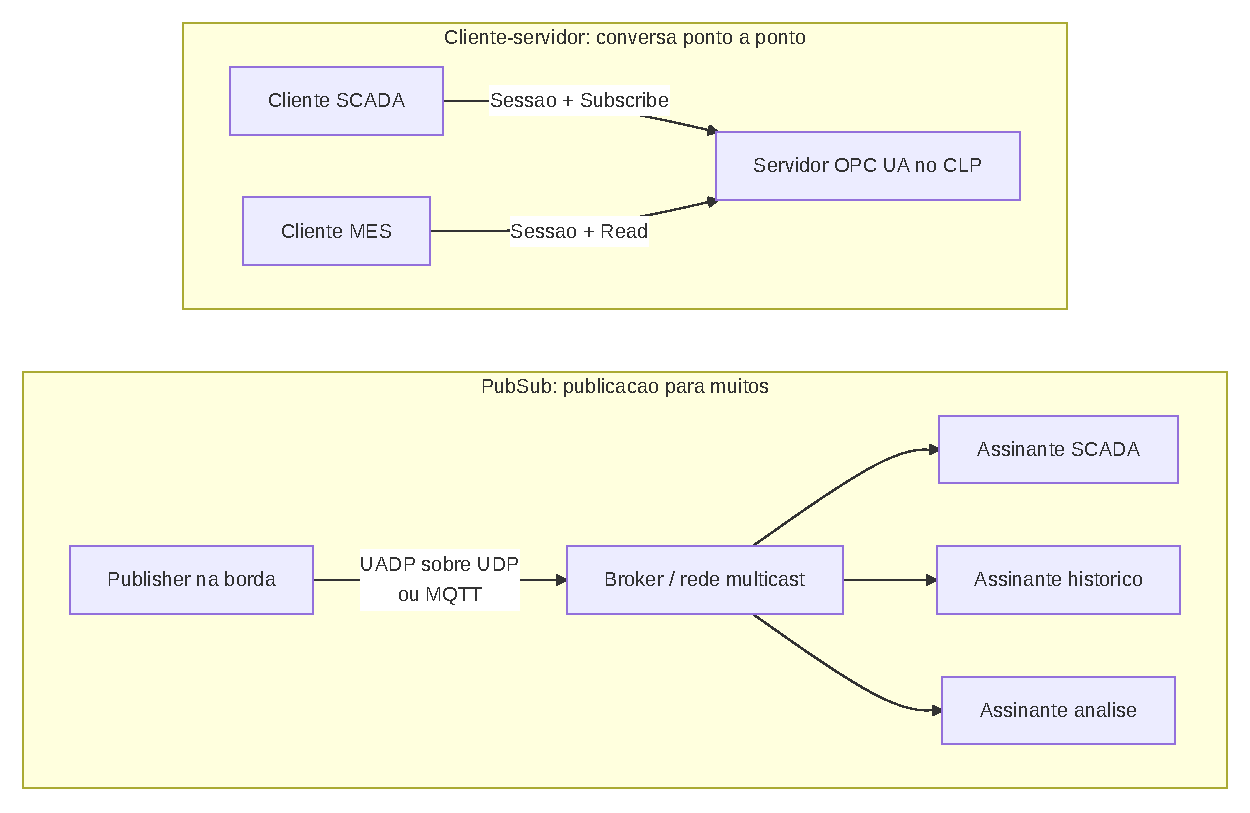
\includegraphics[width=\linewidth,height=0.8\textheight,keepaspectratio]{../figuras/capitulo-13-m2.pdf}%
}{\fbox{\parbox{0.9\linewidth}{\small Diagrama Mermaid ainda não renderizado: capitulo-13-m2. Rode scripts/render-mermaid.sh.}}}
\end{center}

\begin{longtable}[]{@{}
  >{\raggedright\arraybackslash}p{(\columnwidth - 4\tabcolsep) * \real{0.3333}}
  >{\raggedright\arraybackslash}p{(\columnwidth - 4\tabcolsep) * \real{0.3333}}
  >{\raggedright\arraybackslash}p{(\columnwidth - 4\tabcolsep) * \real{0.3333}}@{}}
\toprule\noalign{}
\begin{minipage}[b]{\linewidth}\raggedright
Critério
\end{minipage} & \begin{minipage}[b]{\linewidth}\raggedright
Cliente-servidor
\end{minipage} & \begin{minipage}[b]{\linewidth}\raggedright
PubSub
\end{minipage} \\
\midrule\noalign{}
\endhead
\bottomrule\noalign{}
\endlastfoot
Modelo & Sessão entre cliente e servidor, ponto a ponto & Publicação em rede, muitos assinantes \\
Transporte & \passthrough{\lstinline!opc.tcp!} (porta 4840), HTTPS, WebSocket & UADP sobre UDP, MQTT, AMQP \\
Escala & Boa para supervisão e engenharia & Melhor para muitos consumidores do mesmo dado \\
Latência & Baixa e determinística & Depende do transporte (MQTT acrescenta broker) \\
Uso típico & Diagnóstico, comando, configuração, engenharia & Telemetria em massa, IIoT, integração com nuvem \\
\end{longtable}

A regra prática: \textbf{cliente-servidor para quem conversa com o ativo; PubSub para quem consome o dado em escala.}

\begin{caixafigura}

\textbf{{[}Figura 13.2 -- Espaço de endereços de um servidor OPC UA{]}}
\emph{Captura de um cliente OPC UA genérico mostrando a árvore de nós: Objects \ensuremath{\rightarrow} Servidor \ensuremath{\rightarrow} Bomba 1 \ensuremath{\rightarrow} variáveis com tipo, unidade e valor; ao lado, o painel de atributos do nó selecionado, com StatusCode e SourceTimestamp visíveis. Destacar que a estrutura é descoberta pelo cliente, não digitada em planilha.}

\end{caixafigura}

\begin{center}\rule{0.5\linewidth}{0.5pt}\end{center}

\hypertarget{mqtt}{%
\section{MQTT}\label{mqtt}}

O \textbf{MQTT} (\emph{Message Queuing Telemetry Transport}) é um protocolo publish-subscribe padronizado pela OASIS --- versão \textbf{3.1.1} e versão \textbf{5.0} ---, pensado para enlaces instáveis e dispositivos com poucos recursos.

O desenho é simples: dispositivos \textbf{publicam} em um \textbf{tópico}; o \textbf{broker} entrega a quem \textbf{assinou} aquele tópico (ou um padrão de tópicos). Publisher e subscriber não se conhecem.

\hypertarget{tuxf3picos-e-curingas}{%
\subsection{Tópicos e curingas}\label{tuxf3picos-e-curingas}}

Os tópicos são hierárquicos, separados por \passthrough{\lstinline!/!}:

\begin{lstlisting}
planta/estacao-1/bomba-2/pressao
planta/estacao-1/bomba-2/temperatura
\end{lstlisting}

\begin{longtable}[]{@{}lll@{}}
\toprule\noalign{}
Curinga & Alcance & Exemplo \\
\midrule\noalign{}
\endhead
\bottomrule\noalign{}
\endlastfoot
\passthrough{\lstinline!+!} & Um nível & \passthrough{\lstinline!planta/estacao-1/+/pressao!} \\
\passthrough{\lstinline!\#!} & Todos os níveis abaixo (só no fim) & \passthrough{\lstinline!planta/estacao-1/\#!} \\
\end{longtable}

O tópico é \textbf{contrato de interface}: renomear um nível quebra todos os assinantes silenciosamente. Trate a estrutura de tópicos como se fosse o mapa de registradores do seu Modbus --- documentada e versionada.

\hypertarget{recursos-que-definem-o-comportamento}{%
\subsection{Recursos que definem o comportamento}\label{recursos-que-definem-o-comportamento}}

\begin{longtable}[]{@{}
  >{\raggedright\arraybackslash}p{(\columnwidth - 4\tabcolsep) * \real{0.3333}}
  >{\raggedright\arraybackslash}p{(\columnwidth - 4\tabcolsep) * \real{0.3333}}
  >{\raggedright\arraybackslash}p{(\columnwidth - 4\tabcolsep) * \real{0.3333}}@{}}
\toprule\noalign{}
\begin{minipage}[b]{\linewidth}\raggedright
Recurso
\end{minipage} & \begin{minipage}[b]{\linewidth}\raggedright
O que faz
\end{minipage} & \begin{minipage}[b]{\linewidth}\raggedright
Cuidado prático
\end{minipage} \\
\midrule\noalign{}
\endhead
\bottomrule\noalign{}
\endlastfoot
QoS 0 & Entrega ``no máximo uma vez'' (pode perder) & Aceitável para telemetria de tendência, não para evento \\
QoS 1 & Entrega ``ao menos uma vez'' (pode duplicar) & O assinante precisa ser idempotente \\
QoS 2 & Entrega exatamente uma vez (mais custoso) & Use com parcimônia em enlace de campo \\
\emph{Retained message} & O broker guarda a última mensagem do tópico e a entrega a novos assinantes & Excelente para ``último valor''; perigoso para dado temporal \\
\emph{Last will and testament} (LWT) & Mensagem publicada pelo broker quando o cliente cai & É como se detecta ``dispositivo silencioso'' \\
Sessão persistente & Assinaturas e fila sobrevivem à desconexão & No 5.0 a expiração de sessão é explícita \\
\end{longtable}

A versão 5.0 acrescentou o que faltava para uso industrial: códigos de motivo (\emph{reason codes}), propriedades de usuário, \emph{shared subscriptions} (vários consumidores dividindo a carga de um tópico), apelidos de tópico e expiração de sessão.

\textbf{Tabela 13.2 -- MQTT 3.1.1 \ensuremath{\times} 5.0 (o que muda em projeto industrial)}

\begin{longtable}[]{@{}
  >{\raggedright\arraybackslash}p{(\columnwidth - 4\tabcolsep) * \real{0.3333}}
  >{\raggedright\arraybackslash}p{(\columnwidth - 4\tabcolsep) * \real{0.3333}}
  >{\raggedright\arraybackslash}p{(\columnwidth - 4\tabcolsep) * \real{0.3333}}@{}}
\toprule\noalign{}
\begin{minipage}[b]{\linewidth}\raggedright
Aspecto
\end{minipage} & \begin{minipage}[b]{\linewidth}\raggedright
3.1.1
\end{minipage} & \begin{minipage}[b]{\linewidth}\raggedright
5.0
\end{minipage} \\
\midrule\noalign{}
\endhead
\bottomrule\noalign{}
\endlastfoot
Motivo de falha & Limitado & Códigos de motivo e propriedades \\
Sessão & Binária (limpa ou persistente) & Expiração configurável \\
Escala de consumo & Um assinante por mensagem & \emph{Shared subscriptions} \\
Diagnóstico & Difícil & Propriedades de usuário e fluxo de motivo \\
\end{longtable}

\begin{caixaatencao}

\textbf{Atenção:} MQTT puro não diz \textbf{o que} está no \emph{payload} nem \textbf{de quando} ele é. Um JSON \passthrough{\lstinline!\{"t": 23.4\}!} não informa unidade, ativo nem instante. Sem convenção, cada integração inventa a sua --- e o resultado é o que se vê em muitas plantas: dado na nuvem que ninguém consegue interpretar sem perguntar a quem escreveu o \emph{gateway}.

\end{caixaatencao}

\begin{center}\rule{0.5\linewidth}{0.5pt}\end{center}

\hypertarget{sparkplug-b-mqtt-com-regras}{%
\section{Sparkplug B: MQTT com regras}\label{sparkplug-b-mqtt-com-regras}}

O \textbf{Sparkplug B} é uma especificação mantida pela \textbf{Eclipse Foundation} (versão \textbf{3.0}) que \textbf{define a convenção} que faltava no MQTT industrial: estrutura de tópicos, formato de \emph{payload} e uma máquina de estados para os dispositivos.

\hypertarget{estrutura-de-tuxf3picos}{%
\subsection{Estrutura de tópicos}\label{estrutura-de-tuxf3picos}}

\begin{lstlisting}
spBv1.0/<grupo>/<tipo de mensagem>/<edge node>/[device]
\end{lstlisting}

\begin{longtable}[]{@{}
  >{\raggedright\arraybackslash}p{(\columnwidth - 2\tabcolsep) * \real{0.5000}}
  >{\raggedright\arraybackslash}p{(\columnwidth - 2\tabcolsep) * \real{0.5000}}@{}}
\toprule\noalign{}
\begin{minipage}[b]{\linewidth}\raggedright
Tipo de mensagem
\end{minipage} & \begin{minipage}[b]{\linewidth}\raggedright
Significado
\end{minipage} \\
\midrule\noalign{}
\endhead
\bottomrule\noalign{}
\endlastfoot
\passthrough{\lstinline!NBIRTH!} / \passthrough{\lstinline!NDEATH!} & Nascimento e morte do \emph{edge node}: o que ele publica e quando ele deixa de existir \\
\passthrough{\lstinline!DBIRTH!} / \passthrough{\lstinline!DDEATH!} & Nascimento e morte de um dispositivo subordinado \\
\passthrough{\lstinline!NDATA!} / \passthrough{\lstinline!DDATA!} & Dados do nó e do dispositivo \\
\passthrough{\lstinline!NCMD!} / \passthrough{\lstinline!DCMD!} & Comandos para o nó e para o dispositivo \\
\passthrough{\lstinline!STATE!} & Estado do próprio sistema hospedeiro (online/offline) \\
\end{longtable}

\begin{center}
\IfFileExists{../figuras/capitulo-13-m3.pdf}{%
  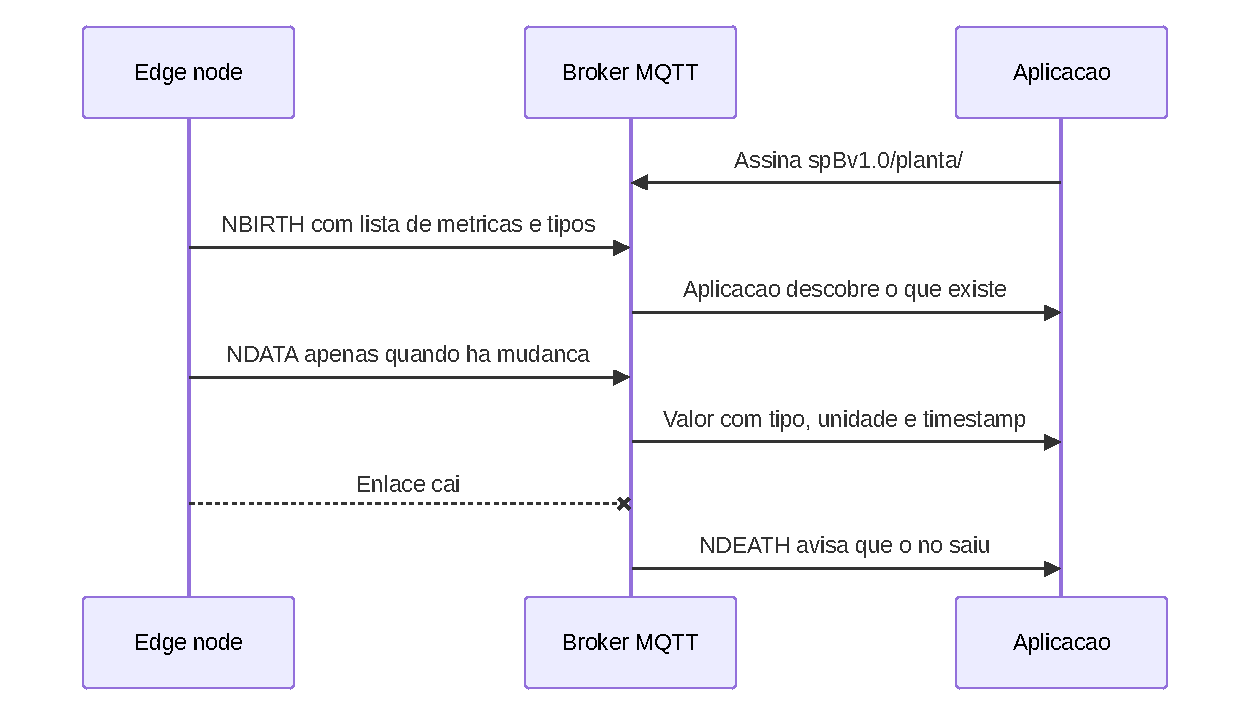
\includegraphics[width=\linewidth,height=0.8\textheight,keepaspectratio]{../figuras/capitulo-13-m3.pdf}%
}{\fbox{\parbox{0.9\linewidth}{\small Diagrama Mermaid ainda não renderizado: capitulo-13-m3. Rode scripts/render-mermaid.sh.}}}
\end{center}

O ganho é direto:

\begin{itemize}
\tightlist
\item
  \textbf{\passthrough{\lstinline!NBIRTH!} entrega o dicionário de dados.} O consumidor descobre nomes, tipos e unidades das métricas sem planilha externa.
\item
  \textbf{\passthrough{\lstinline!NDEATH!}/\passthrough{\lstinline!DDEATH!}} resolvem a detecção de dispositivo offline de forma explícita (é o LWT organizado).
\item
  \textbf{Publicação por exceção} (\emph{report by exception}): publica quando muda, reduzindo tráfego de enlace caro.
\item
  \textbf{Payload com tipo e \emph{timestamp} por métrica} --- resolve o problema do ``número sem contexto''.
\item
  \textbf{Número de sequência} permite detectar perda de mensagens.
\end{itemize}

\hypertarget{o-que-o-sparkplug-nuxe3o-resolve}{%
\subsection{\texorpdfstring{O que o Sparkplug \textbf{não} resolve}{O que o Sparkplug não resolve}}\label{o-que-o-sparkplug-nuxe3o-resolve}}

\begin{itemize}
\tightlist
\item
  Não é controle: não é protocolo de malha fechada nem de segurança funcional.
\item
  Não substitui o OPC UA para descoberta rica de estrutura, métodos e histórico em equipamento que já fala OPC UA.
\item
  Não dispensa a disciplina de modelagem: um sistema Sparkplug mal nomeado continua sendo um sistema difícil de integrar.
\end{itemize}

\begin{center}\rule{0.5\linewidth}{0.5pt}\end{center}

\hypertarget{combinando-as-truxeas-peuxe7as}{%
\section{Combinando as três peças}\label{combinando-as-truxeas-peuxe7as}}

Na prática, os protocolos se sobrepõem em papéis diferentes:

\textbf{Tabela 13.3 -- Comparação para decisão de projeto}

\begin{longtable}[]{@{}
  >{\raggedright\arraybackslash}p{(\columnwidth - 6\tabcolsep) * \real{0.2500}}
  >{\raggedright\arraybackslash}p{(\columnwidth - 6\tabcolsep) * \real{0.2500}}
  >{\raggedright\arraybackslash}p{(\columnwidth - 6\tabcolsep) * \real{0.2500}}
  >{\raggedright\arraybackslash}p{(\columnwidth - 6\tabcolsep) * \real{0.2500}}@{}}
\toprule\noalign{}
\begin{minipage}[b]{\linewidth}\raggedright
Critério
\end{minipage} & \begin{minipage}[b]{\linewidth}\raggedright
OPC UA cliente-servidor
\end{minipage} & \begin{minipage}[b]{\linewidth}\raggedright
MQTT 5.0
\end{minipage} & \begin{minipage}[b]{\linewidth}\raggedright
Sparkplug B sobre MQTT
\end{minipage} \\
\midrule\noalign{}
\endhead
\bottomrule\noalign{}
\endlastfoot
Descoberta de estrutura & Completa (espaço de endereços) & Nenhuma & Dicionário no \passthrough{\lstinline!NBIRTH!} \\
Semântica do dado & Tipos, unidades, \emph{status code} & Definida pelo usuário & Métrica tipada no \emph{payload} \\
Segurança & Nativa (X.509, políticas) & TLS no transporte + credenciais & Herdada do MQTT/TLS \\
Comando & Serviços e métodos & Tópico de comando (livre) & \passthrough{\lstinline!NCMD!}/\passthrough{\lstinline!DCMD!} padronizados \\
Escala de consumidores & Sessão por cliente & Alta, com \emph{shared subscriptions} & Alta \\
Melhor uso & Equipamento, engenharia, comando & Telemetria, integração, nuvem & IIoT padronizado, frota de \emph{gateways} \\
Limitação típica & Mais pesado na borda & Sem semântica & Menos flexível que OPC UA \\
\end{longtable}

\begin{center}
\IfFileExists{../figuras/capitulo-13-m4.pdf}{%
  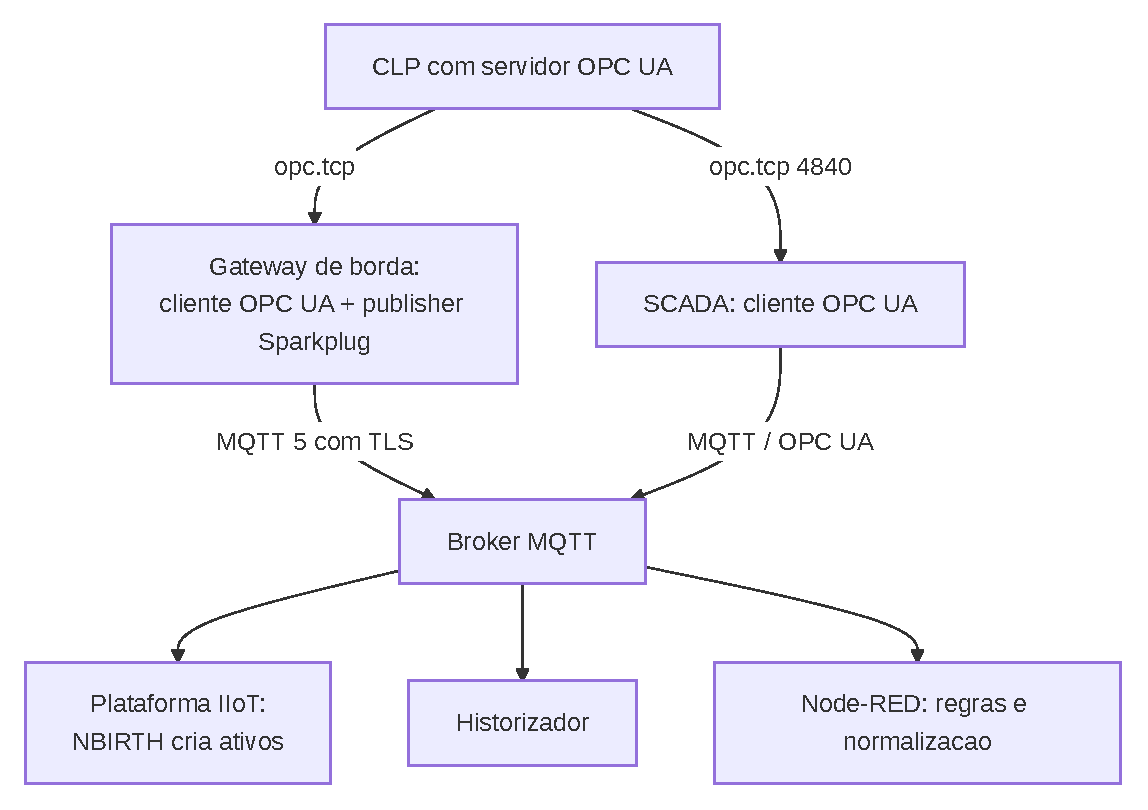
\includegraphics[width=\linewidth,height=0.8\textheight,keepaspectratio]{../figuras/capitulo-13-m4.pdf}%
}{\fbox{\parbox{0.9\linewidth}{\small Diagrama Mermaid ainda não renderizado: capitulo-13-m4. Rode scripts/render-mermaid.sh.}}}
\end{center}

\begin{caixanota}

\textbf{Atualização tecnológica:} este capítulo não existia no material original, que tratava OPC UA e MQTT apenas como ``protocolos modernos'' em um subtópico. A separação entre transporte, semântica e comportamento --- e o papel do Sparkplug B como convenção --- refletem a prática atual de projetos de integração industrial. As fontes estão citadas ao final.

\end{caixanota}

\begin{caixafigura}

\textbf{{[}Figura 13.3 -- Arquitetura de integração com OPC UA e Sparkplug B{]}}
\emph{Diagrama em camadas: à esquerda o CLP com servidor OPC UA (endpoint e política de segurança anotados); no centro o gateway de borda com as duas funções destacadas (cliente OPC UA e publisher Sparkplug); à direita o broker e os consumidores (SCADA, historizador, plataforma, Node-RED). Anotar o sentido das setas e marcar com cadeado o trecho cifrado.}

\end{caixafigura}

\begin{center}\rule{0.5\linewidth}{0.5pt}\end{center}

\hypertarget{estudo-de-caso-integrauxe7uxe3o-de-uma-frota-de-gateways}{%
\section{\texorpdfstring{Estudo de caso --- integração de uma frota de gateways}{Estudo de caso  integração de uma frota de gateways}}\label{estudo-de-caso-integrauxe7uxe3o-de-uma-frota-de-gateways}}

\begin{caixafigura}

\textbf{{[}Figura 13.4 -- Tela de configuração do publisher Sparkplug no gateway de borda{]}}
\emph{Captura de uma interface de configuração de gateway (genérica, sem marca) com: endereço do broker e porta, TLS habilitado e certificado carregado, \passthrough{\lstinline!group id!} e \passthrough{\lstinline!edge node id!}, intervalo de publicação e }deadband* por métrica, e a lista de métricas mapeadas com nome, tipo e unidade. Destacar a área onde aparece o \passthrough{\lstinline!NBIRTH!} publicado e o estado da conexão.*

\end{caixafigura}

\textbf{Cenário.} Cinco subestações de distribuição de água, cada uma com um CLP e um \emph{gateway} de borda. O SCADA central precisa de supervisão em tempo real; a engenharia precisa de histórico; a gestão precisa de indicadores; e a manutenção precisa saber quando um \emph{gateway} cai. O enlace é 4G, com franquia de dados.

\textbf{Decisão de arquitetura.}

\begin{longtable}[]{@{}
  >{\raggedright\arraybackslash}p{(\columnwidth - 4\tabcolsep) * \real{0.3333}}
  >{\raggedright\arraybackslash}p{(\columnwidth - 4\tabcolsep) * \real{0.3333}}
  >{\raggedright\arraybackslash}p{(\columnwidth - 4\tabcolsep) * \real{0.3333}}@{}}
\toprule\noalign{}
\begin{minipage}[b]{\linewidth}\raggedright
Necessidade
\end{minipage} & \begin{minipage}[b]{\linewidth}\raggedright
Solução
\end{minipage} & \begin{minipage}[b]{\linewidth}\raggedright
Por quê
\end{minipage} \\
\midrule\noalign{}
\endhead
\bottomrule\noalign{}
\endlastfoot
Supervisão do CLP em tempo real & OPC UA cliente-servidor, assinatura com \emph{deadband} & Descoberta de estrutura, \emph{status code} e controle de tráfego \\
Telemetria agregada para a nuvem & Sparkplug B sobre MQTT 5 com TLS & Dicionário no \passthrough{\lstinline!NBIRTH!}, publicação por exceção, detecção de queda \\
Detecção de \emph{gateway} offline & \passthrough{\lstinline!NDEATH!} + monitoramento do broker & Não depende de alguém perceber o dado parado \\
Comando de \emph{setpoint} & OPC UA \passthrough{\lstinline!Write!} autenticado, com registro de auditoria & Comando exige controle de acesso e trilha \\
Histórico & Historizador assinando OPC UA e consumindo MQTT & Duas fontes, mesma modelagem de nomes \\
\end{longtable}

\textbf{Regras adotadas.}

\begin{enumerate}
\def\labelenumi{\arabic{enumi}.}
\tightlist
\item
  \textbf{Um único dicionário de nomes.} O mesmo identificador de ativo e de variável vale no espaço de endereços do OPC UA, no tópico Sparkplug e no historizador. Sem isso, o relatório da gestão e o sinótico do operador falam línguas diferentes.
\item
  \textbf{Política de segurança obrigatória} no OPC UA e \textbf{TLS} no MQTT, com certificados renovados no calendário de manutenção.
\item
  \textbf{Agregação na borda:} amostragem de 1 s no CLP, publicação por exceção com \emph{deadband} --- consumo de dados reduzido a menos de um décimo do que seria com publicação periódica de tudo.
\item
  \textbf{\passthrough{\lstinline!StatusCode!} propagado até a tela.} Variável com qualidade ruim aparece como tal, e não como valor zero.
\item
  \textbf{Sem comando pela nuvem.} O comando de \emph{setpoint} sai do SCADA por OPC UA; a nuvem é somente leitura. É a aplicação direta da regra do Capítulo 12.
\end{enumerate}

\textbf{Resultado.} A manutenção passou a ver a queda de um \emph{gateway} em segundos (pelo \passthrough{\lstinline!NDEATH!}), em vez de descobrir a falha no dia seguinte pela ausência de dados. O diagnóstico de sensor com defeito deixou de ser confundido com ``pressão zero''. E o consumo de dados caiu o suficiente para manter o enlace 4G dentro da franquia.

\begin{center}\rule{0.5\linewidth}{0.5pt}\end{center}

\hypertarget{atividade-pruxe1tica}{%
\section{Atividade prática}\label{atividade-pruxe1tica}}

\begin{enumerate}
\def\labelenumi{\arabic{enumi}.}
\tightlist
\item
  Suba um servidor OPC UA de teste (por exemplo, um simulador público de servidor OPC UA) e navegue pelo espaço de endereços com um cliente genérico.
\item
  Escolha três variáveis e monte uma assinatura com \emph{sampling interval} de 1 s e \emph{deadband} de 0,5\%. Compare o número de notificações com e sem \emph{deadband}.
\item
  Verifique quais políticas de segurança o servidor anuncia e tente conectar com \passthrough{\lstinline!SecurityPolicy: None!}. Registre o que aconteceu e o risco correspondente.
\item
  Publique a mesma telemetria em MQTT com QoS 0 e QoS 1; simule queda de enlace e compare o que o assinante recebe.
\item
  Estruture os tópicos conforme Sparkplug B para um \emph{edge node} com dois dispositivos e simule \passthrough{\lstinline!NBIRTH!}, \passthrough{\lstinline!NDATA!} e \passthrough{\lstinline!NDEATH!}.
\item
  Escreva, em uma página, o dicionário de dados (ativo, variável, tipo, unidade, faixa, regra de qualidade) usado nos itens anteriores. Esse documento é o produto mais importante da atividade.
\end{enumerate}

\begin{center}\rule{0.5\linewidth}{0.5pt}\end{center}

\hypertarget{resumo}{%
\section{Resumo}\label{resumo}}

\begin{itemize}
\tightlist
\item
  Conectar é transporte; \textbf{integrar é semântica}. A maior parte das falhas de integração é falta de modelagem, não de protocolo.
\item
  \textbf{OPC UA} (OPC Foundation, 2008; série IEC 62541) oferece espaço de endereços, tipos, \emph{status code}, assinatura com \emph{deadband}, métodos e segurança nativa com X.509.
\item
  Modos de segurança \passthrough{\lstinline!None!}, \passthrough{\lstinline!Sign!} e \passthrough{\lstinline!SignAndEncrypt!}: escolher \passthrough{\lstinline!None!} em rede compartilhada é expor leitura e escrita.
\item
  \textbf{Cliente-servidor} atende quem conversa com o ativo; \textbf{PubSub} atende muitos consumidores do mesmo dado.
\item
  \textbf{MQTT} (OASIS 3.1.1 e 5.0) é publish-subscribe com QoS 0/1/2, \emph{retained}, \emph{last will} e, na versão 5.0, códigos de motivo e \emph{shared subscriptions} --- mas \textbf{não define o conteúdo}.
\item
  \textbf{Sparkplug B 3.0} (Eclipse Foundation) define tópicos, \emph{payload} tipado, \passthrough{\lstinline!NBIRTH!}/\passthrough{\lstinline!NDEATH!} e publicação por exceção: é o MQTT com regras de interoperabilidade.
\item
  A combinação típica é OPC UA para equipamento e comando, MQTT/Sparkplug para telemetria em escala, e um \textbf{dicionário de nomes único} atravessando SCADA, historizador e plataforma.
\item
  Nenhuma dessas tecnologias substitui CLP e SCADA em controle, proteção e segurança funcional.
\end{itemize}

\hypertarget{questuxf5es-de-revisuxe3o}{%
\section{Questões de Revisão}\label{questuxf5es-de-revisuxe3o}}

\begin{enumerate}
\def\labelenumi{\arabic{enumi}.}
\tightlist
\item
  Explique a diferença entre transporte e semântica, com um exemplo de falha causada pela ausência de semântica.
\item
  O que é o espaço de endereços do OPC UA e por que o cliente descobre a estrutura em vez de receber um mapa?
\item
  Qual a função do \passthrough{\lstinline!StatusCode!} e o que acontece se ele for ignorado na tela do operador?
\item
  Compare \passthrough{\lstinline!SecurityPolicy: None!}, \passthrough{\lstinline!Sign!} e \passthrough{\lstinline!SignAndEncrypt!} quanto à garantia oferecida.
\item
  Em que situação o OPC UA PubSub é preferível ao cliente-servidor? Justifique com um exemplo de planta.
\item
  Descreva o papel do broker MQTT e por que publisher e subscriber não precisam se conhecer.
\item
  Explique QoS 0, 1 e 2 com um caso de uso industrial para cada, indicando o risco de escolher mal.
\item
  O que um \emph{retained message} resolve e qual é o seu risco quando o dado é temporal?
\item
  O que o Sparkplug B acrescenta ao MQTT? Cite três elementos concretos da especificação.
\item
  Uma planta quer publicar 500 variáveis a cada 100 ms na nuvem, por enlace 4G com franquia. Critique a proposta e proponha uma arquitetura alternativa com OPC UA e Sparkplug.
\end{enumerate}

\hypertarget{referuxeancias}{%
\section{Referências}\label{referuxeancias}}

\begin{itemize}
\tightlist
\item
  OPC FOUNDATION. \textbf{OPC Unified Architecture} --- conceitos, modelo de informação, serviços, segurança e especificação PubSub. Disponível em: opcfoundation.org. Consulta: 2026.
\item
  INTERNATIONAL ELECTROTECHNICAL COMMISSION. \textbf{IEC 62541 --- OPC Unified Architecture} (série; verificar edição vigente).
\item
  OASIS. \textbf{MQTT Version 3.1.1} (2014) e \textbf{MQTT Version 5.0} (2019) --- especificações do protocolo. Disponível em: docs.oasis-open.org.
\item
  ECLIPSE FOUNDATION. \textbf{Sparkplug Specification 3.0} --- estrutura de tópicos, \emph{payload} e máquina de estados. Disponível em: \url{eclipse.org/tahu}.
\item
  MATERIAL DE ORIGEM: \emph{Livro SCADA --- versão para análise} (integração de sistemas e protocolos;
  figura da arquitetura lógica OPC dos autores, reproduzida com crédito);
  \passthrough{\lstinline!Node-Red\_InterfaceDeSupervisão.pdf!} (cliente OPC UA e MQTT no Node-RED); \passthrough{\lstinline!IoT.pdf!} e
  \passthrough{\lstinline!IIoT e suas Tecnologias Aderentes.pdf!} (protocolos de IIoT).
\end{itemize}
